% +------------------------------------------------------------------------+
% | Reference manual page: Delaunay_triangulation_3.tex
% +------------------------------------------------------------------------+
% | 27.3.2000   Monique Teillaud
% | Package: Triangulation3
% | 
\RCSdef{\RCSDelaunaytriangulationRev}{$Revision$}
\RCSdefDate{\RCSDelaunaytriangulationDate}{$Date$}
% |
%%RefPage: end of header, begin of main body
% +------------------------------------------------------------------------+


\begin{ccRefClass}{Delaunay_triangulation_3<Triangulation_traits_3,Tds_3>}  %% add template arg's if necessary

%% \ccHtmlCrossLink{}     %% add further rules for cross referencing links
%% \ccHtmlIndexC[class]{} %% add further index entries

\ccDefinition
  
The class \ccRefName\ represents a three-dimensional Delaunay triangulation.

\ccInclude{CGAL/Delaunay_triangulation_3.h}

\ccInheritsFrom{\ccc{Triangulation_3<Triangulation_traits_3,Tds_3>}}

\ccTypes

Inherits the types of \ccc{Triangulation_3<Triangulation_traits_3,Tds_3>}.

\ccCreation
\ccCreationVariable{dt}  %% choose variable name
\ccThree{Vertex_handle}{dt.remove(Pont p)toto}{}

\ccConstructor{Delaunay_triangulation_3();}{default constructor.}


\ccConstructor{Delaunay_triangulation_3<Triangulation_traits_3,Tds_3>()}
{Creates an empty Delaunay triangulation.}

\ccConstructor{Delaunay_triangulation_3<Triangulation_traits_3,Tds_3>
(const Triangulation_traits_3 & traits)}
{Creates an empty Delaunay triangulation with traits class
\ccc{traits}.}

\ccConstructor{Delaunay_triangulation_3<Triangulation_traits_3,Tds_3>
(const Delaunay_triangulation_3<Triangulation_traits_3,Tds_3> & dt1)}
{Copy constructor.}

\ccOperations

\ccHeading{Insertion}

The following methods overload the corresponding methods of
triangulations to ensure the empty sphere property of Delaunay 
triangulations.

\ccMethod{Vertex_handle insert(const Point & p );}
{Inserts point \ccc{p} in the triangulation and returns the corresponding
 vertex. Similar to the insertion in a triangulation, but ensures in
addition the empty sphere property of all the created faces.}

\ccMethod{Vertex_handle insert(const Point & p, Cell_handle start);}
{Same as the previous method, \ccc{start} is used as a starting
place for the search done within the insertion.}

The following method allows one to insert several points. It returns the
number of inserted points. 

\ccMethod{template < class InputIterator >
          int
          insert(InputIterator first, InputIterator last);}
{Inserts the points in the range $\left[\right.$\ccc{first},
\ccc{last}$\left.\right)$. 
\ccPrecond{The \ccc{value_type} of \ccc{first} and \ccc{last} is
\ccc{Point}.}}
%\ccMethod{int insert(list<Point>::const_iterator first,
%	     list<Point>::const_iterator last);}
%{}
%\ccGlue
%\ccMethod{int insert(vector<Point>::const_iterator first,
%	     vector<Point>::const_iterator last);}
%{}
%\ccGlue
%\ccMethod{int insert(istream_iterator<Point, ptrdiff_t> first,
%	     istream_iterator<Point, ptrdiff_t> last);}
%{}
%\ccGlue
%\ccMethod{int insert(Point* first,
%	     Point* last);}
%{}

\ccHeading{Removal}

When a vertex \ccc{v} is removed from a triangulation, all the cells
incident to \ccc{v} must be removed, and the polyhedral region
consisting of all the tetrahedra that are incident to \ccc{v} must be
retriangulated. 

So, the problem reduces to triangulating a polyhedral
region, while preserving its boundary, or to compute a
\textit{constrained} triangulation. This is known to be sometimes
impossible: the Sch\"onhardt polyhedron cannot be triangulated
\cite{s-cgehd-98}. 

However, when dealing with Delaunay triangulations, the case of such
polyhedra that cannot be retriangulated ``cannot'' happen, and a very
efficient algorithm was recently proposed \cite{d-ddt-99} and
implemented. At least, this is what is commonly thought. The algorithm 
just cited uses symbolic perturbations, so that degeneracies do not
appear, whereas \cgal\ explicitly treats all degenerate cases.
Suppose for instance that the hole created consists of cospherical
points, some of them being coplanar.
Figure~\ref{Triangulation3-fig-remimpos} shows the simplest
realization of this case. Then it is \textit{impossible} to
triangulate the interior of the polyhedron without creating edges that
intersect already existing edges.

\begin{figure}[htbp]
\begin{ccTexOnly}
\begin{center} 
\includegraphics{remimpos.eps} 
\end{center}
\end{ccTexOnly}
\caption{Removal is impossible in some degenerate cases.
\label{Triangulation3-fig-remimpos}}
\begin{ccHtmlOnly}
<CENTER>
<img border=0 src="./remimpos.gif" align=center alt="Removal is impossible in some degenerate cases">
</CENTER>
\end{ccHtmlOnly}
\end{figure} 

It may be possible in such a case to modify the triangulation outside
the hole so that it becomes consitent with a triangulation of the
interior of the hole, but it might turn out that the whole
triangulation has to be modified, for some very degenerate cases such
as data points being the vertices of a regular grid. Finding an
algorithm that modifies the minimum number of cells is an open problem.

Anyway, \cgal\ proposes a method that removes a vertex if it is
possible. If it is not possible, the current implementation tries to
remove the vertex, and returns \ccc{false} as soon as it finds a facet
that cannot form a tetrahedron inside the hole with any other vertex
of the hole. The drawback is that the triangulation is then completely
invalidated and cannot be restored in its previous state. The user
dealing with very degenerate input data might want to copy his
triangulation before trying to remove a vertex.

In practical cases, the probability that such a problem arises is
of course very low.

\ccMethod{bool remove(Vertex_handle v);}
{Removes the vertex \ccc{v} from the triangulation and returns
\ccc{true}, if it is possible. Otherwise, it returns false.
\ccPrecond{\ccc{v} is a vertex of the triangulation and it is not the
infinite vertex}}

\ccHeading{Queries}

\ccMethod{Bounded_side
          side_of_sphere(Cell_handle c, const Point & p) const;}
{Returns a value indicating on which side of the circumscribed sphere
of \ccc{c} the point \ccc{p} lies. More precisely, it returns:\\
- \ccc{ON_BOUNDED_SIDE} if \ccc{p} is inside the sphere. For an infinite
cell this means that \ccc{p} lies strictly either in the half space
limited by its finite facet and not containing any other point of the
triangulation, or in the interior of the disk circumscribing the
\textit{finite} facet. \\ 
- \ccc{ON_BOUNDARY} if p on the boundary of the sphere. For an infinite
cell this means that \ccc{p} lies on the circle circumscribing
the \textit{finite} facet.\\ 
- \ccc{ON_UNBOUNDED_SIDE} if \ccc{p} lies outside the sphere. For an
infinite cell this means that \ccc{p} does not satisfy either of the
two previous conditions. 
\ccPrecond{\ccVar.\ccc{dimension()} $=3$.}}
\ccMethod{Bounded_side
	  side_of_circle(const Facet & f, const Point & p) const;}
{Returns a value indicating on which side of the circumscribed circle
of \ccc{f} the point \ccc{p} lies. More precisely, it returns:\\
- in dimension~3:\\
-- For a finite facet, \ccc{ON_BOUNDARY} if \ccc{p} lies
on the circle, \ccc{ON_UNBOUNDED_SIDE} when it lies in the exterior of
the disk, \ccc{ON_BOUNDED_SIDE} when it lies in its interior.\\
-- For an infinite facet, it considers the plane defined by the finite
facet of the same cell, and does the same as in dimension~2 in this
plane.\\
- in dimension~2:\\
-- For a finite facet, \ccc{ON_BOUNDARY} if \ccc{p} lies
on the circle, \ccc{ON_UNBOUNDED_SIDE} when it lies in the exterior of
the disk, \ccc{ON_BOUNDED_SIDE} when it lies in its interior.\\
-- For an infinite facet, \ccc{ON_BOUNDARY} if the
point lies on the finite edge of \ccc{f} (endpoints included),
\ccc{ON_BOUNDED_SIDE} for a point in the open half plane defined
by \ccc{f} and not containing any other point of the triangulation,
\ccc{ON_UNBOUNDED_SIDE} elsewhere. 
\ccPrecond{\ccVar.\ccc{dimension()} $\geq 2$ and in dimension 3,
\ccc{p} is coplanar with \ccc{f}.}}

\ccMethod{Bounded_side
	  side_of_circle(Cell_handle c, int i, const Point & p);}
{Same as the previous method for facet \ccc{i} of cell \ccc{c}.}

\begin{ccAdvanced}
\ccHeading{Checking}
\ccMethod{bool
          is_valid(bool verbose = false) const;}
{Checks the combinatorial validity of the triangulation and the
validity of its geometric embedding (see
Section~\ref{Triangulation3-sec-Valid}). Also checks that all the
circumscribing spheres (resp. circles in dimension~2) of  cells
(resp. facets in dimension~2) are empty.\\ When \ccc{verbose} is set to
true,  messages describing the first invalidity encountered are
printed.}

\ccMethod{bool
          is_valid(Cell_handle c, bool verbose = false) const;}
{Checks the combinatorial and geometric validity of the cell (see
Section~\ref{Triangulation3-sec-Valid}). Also checks that the
circumscribing sphere (resp. circle in dimension~2) of  cells
(resp. facet in dimension~2) is empty.\\
 When \ccc{verbose} is set to
true, messages are printed to give
a precise indication of the kind of invalidity encountered.}

These methods are  mainly a debugging help for the users of advanced features.
\end{ccAdvanced}

\ccSeeAlso

\ccc{CGAL::Delaunay_hierarchic_triangulation_3<Triangulation_traits_3,Tds_3>}.

%% \ccExample

%% \ccIncludeExampleCode{examples/Triangulation3/Delaunay_triangulation_3_prog.C}

\end{ccRefClass}

% +------------------------------------------------------------------------+
%%RefPage: end of main body, begin of footer
% EOF
% +------------------------------------------------------------------------+

